\documentclass[a4paper, 12pt]{article}

%\usepackage{cmap}
\usepackage[T2A]{fontenc}
\usepackage[utf8]{inputenc}
\usepackage[english, russian]{babel}
\usepackage{graphicx}
\usepackage[top=1in, bottom=1in, left=3.2cm, right=2.6cm]{geometry}
\graphicspath{./}
\usepackage{biblatex}
\addbibresource{lib.bib}
\linespread{1.5}
\usepackage{ragged2e}
\justifying
\usepackage{listings}
\usepackage{color}
\usepackage{amsmath}


\begin{document}
	
\begin{titlepage}
	\fontsize{12pt}{12pt}\selectfont
	\begin{figure}[t!]
		\centering
		
\includegraphics[scale=0.8]{bmstu}
	\end{figure}
	
	\noindent\rule{15cm}{3pt}
	\newline\newline
	\noindent 
	ФАКУЛЬТЕТ 
	\underline{«Информатика и системы управления»} \newline
	
	\noindent КАФЕДРА \underline{«Программное обеспечение ЭВМ и информационные технологии»}\newline\newline\newline\newline\newline
	
	\centering {\Large \textbf{Отчет по лабораторной работе № 3}}
	\vspace{4mm}
	
	\centering {\Large \textbf{По курсу:} Моделирование
		\vspace{8mm}}
	\\ \centering {\Large \textbf{На тему:} Генераторы псевдослучайных чисел}
	\vspace{20mm}
	
	
	\begin{flushright}
		{\small	\textbf{Студент:}\\ Турсунов Жасурбек Рустамович \\ \textbf{Группа:} ИУ7-76Б
			\vspace{3mm}
			\\\textbf{Преподователь:} \\ Рудаков Игорь Владимирович }
	\end{flushright}
	
	\begin{center}
		\vfill
		Москва, \the\year
		~г.
	\end{center}
\end{titlepage}

\tableofcontents
\clearpage
\newpage


\section{{Задание}}

\hspace*{5mm} Изучить и реализовать генератор псевдослучайных чисел программным и табличным методом. Разрядность чисел должна быть равна 1, 2, 3. Сравнить методы по определенному критерию и сделать выводы.

\section{{Теоритическая часть}}
\hspace*{5mm} В данной лаборатоной работе рассматриваются 2 метода генерации случайных чисел:
\begin{enumerate}
	\item программный;
	\item табличный.
\end{enumerate}
\subsection{Программный генератор}
\hspace*{5mm} Программный генератор формирует псевдослучайные числа. Каждое последующее число в такой последовательности зависит от предыдущего.

\subsection{Табличный генератор}
\hspace*{5mm} Табличный генератор использует таблицу проверенных некоррелированных цифр в качестве источника случайных чисел.
\subsection{Критерий случайности}
\hspace*{5mm} Для сравнения описанных методов генерации случайных чисел воспользуемся \textbf{критерием частотности}, который позволяет определить равномерность сгенерированных чисел.

\hspace*{5mm} Определяется количество чисел на интервале $(\mu - \sigma,\ \mu + \sigma)$, где $\mu$~--- математическое ожидание, а $\sigma$~--- среднеквадратичное отклонение. Идеальным результатом будем считать отношение длины рассматриваемого интервала к длине всего промежутка, на котором генерируется последовательность. Под полученным результатом будем понимать отношение количества сгенерированных чисел на интервале к количеству всех сгенерированных чисел.


\section{{Результаты}}
\begin{figure}[h!]
	\centering 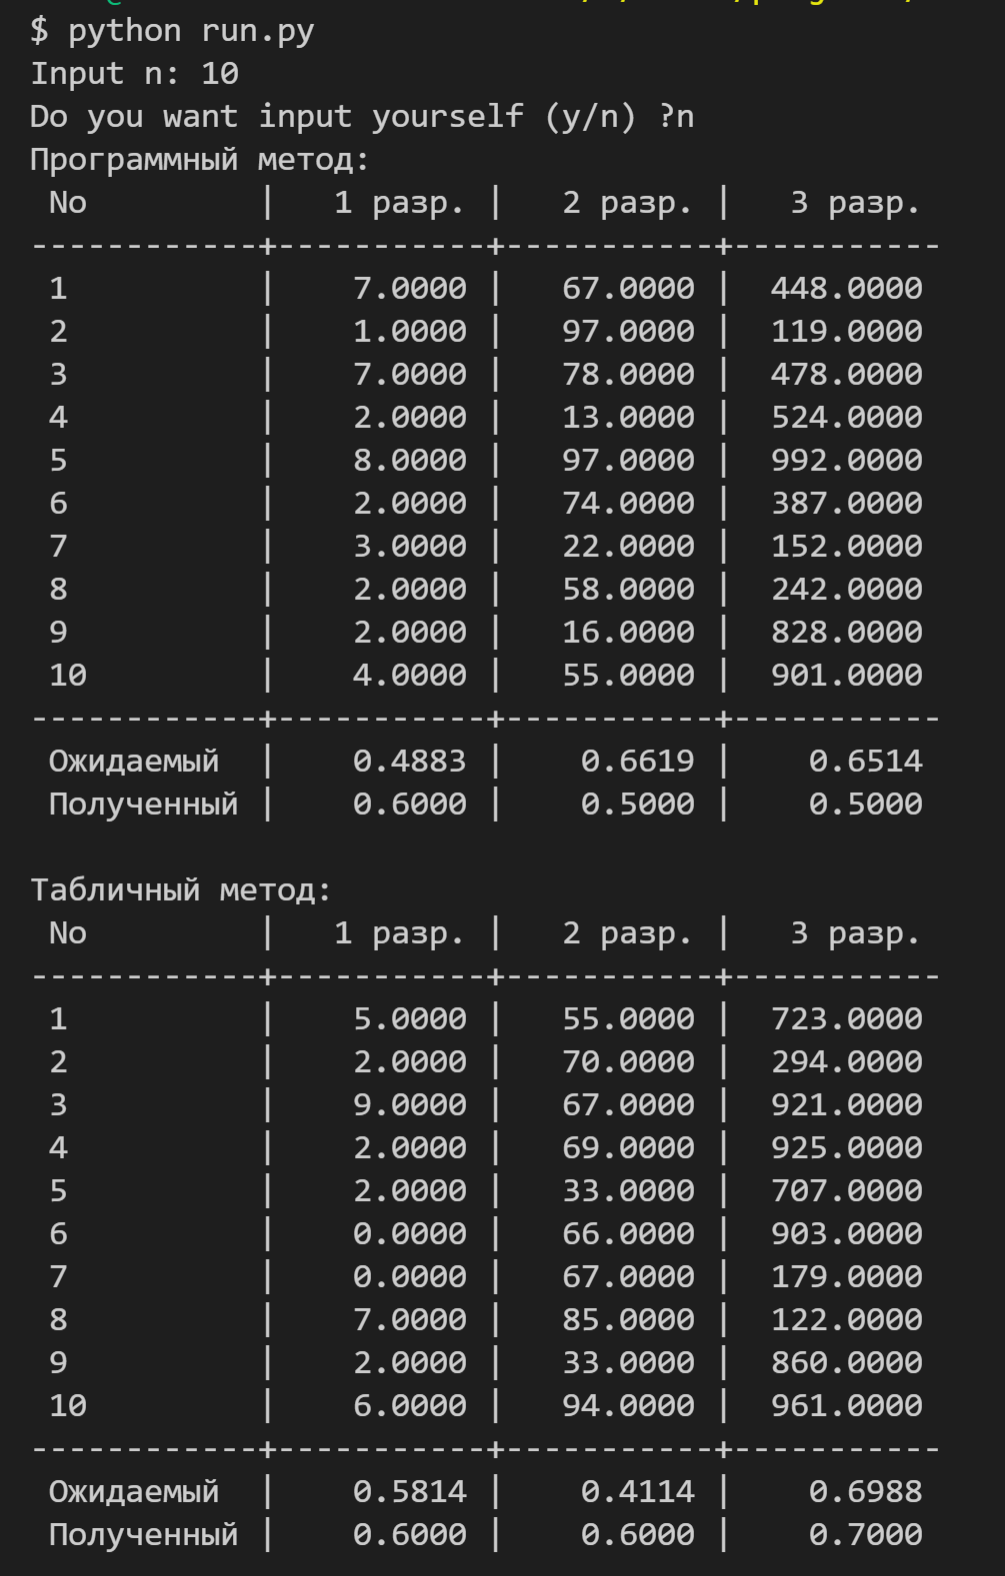
\includegraphics[scale=1]{10}
	\centering\caption{Пример работы для 10 чисел}
\end{figure}
\clearpage
\newpage
\begin{figure}[t!]
	\centering 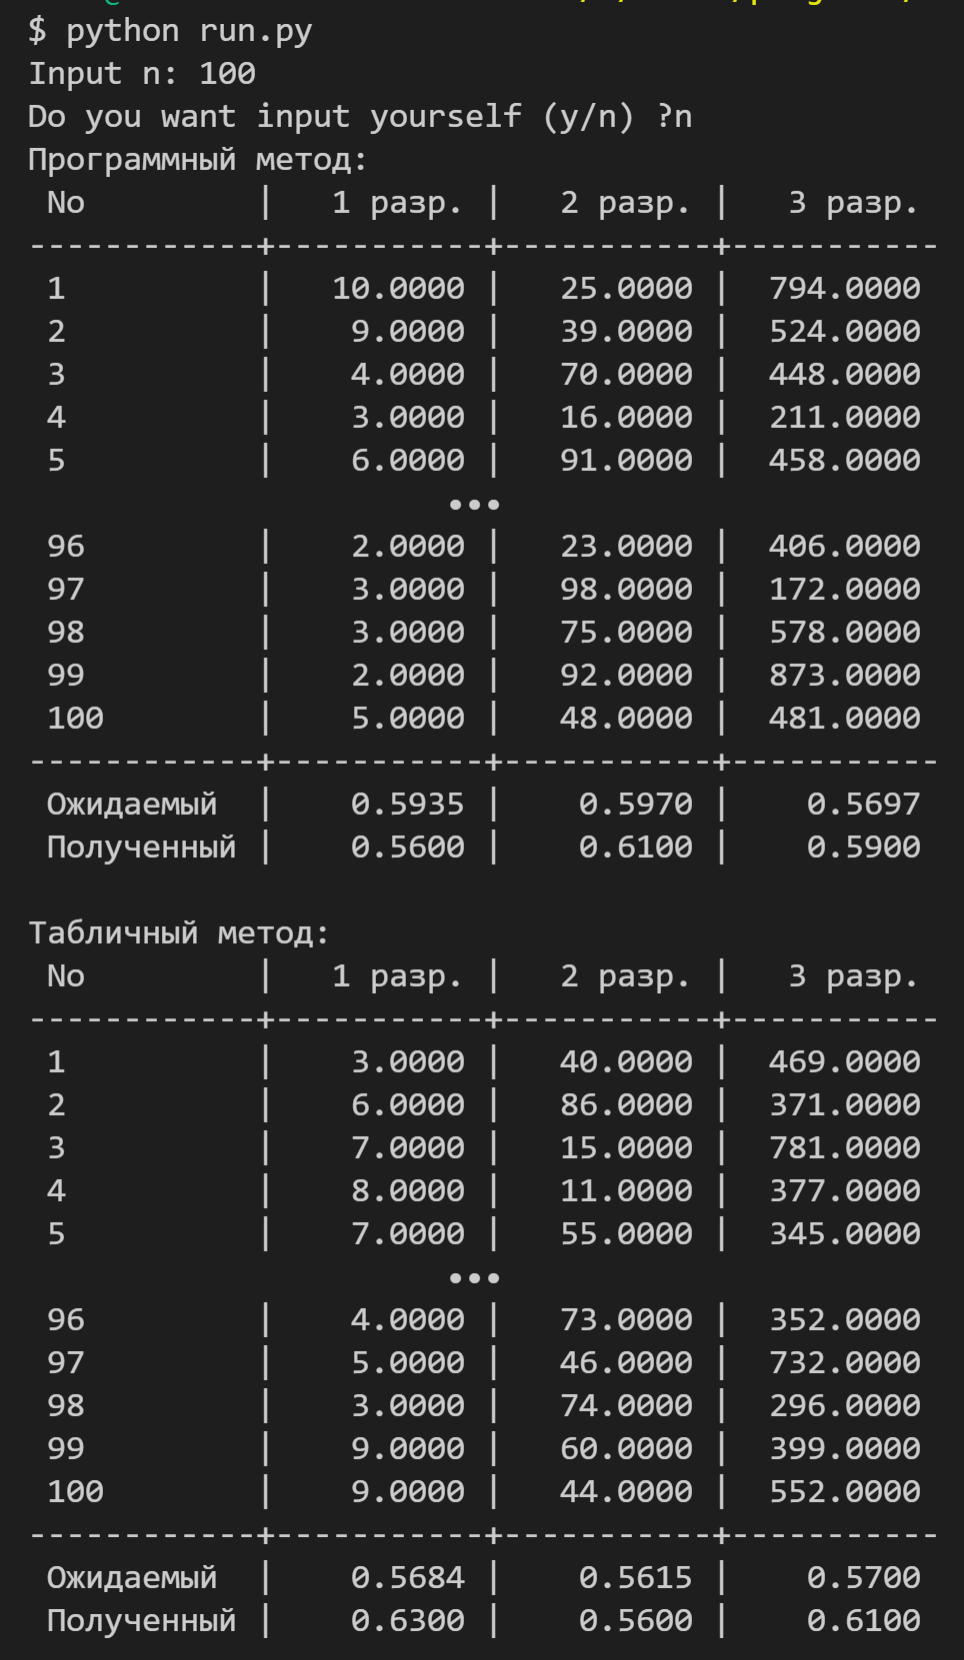
\includegraphics[scale=1]{100}
	\centering\caption{Пример работы для 100 чисел}
\end{figure}
\clearpage
\newpage
\begin{figure}[t!]
	\centering 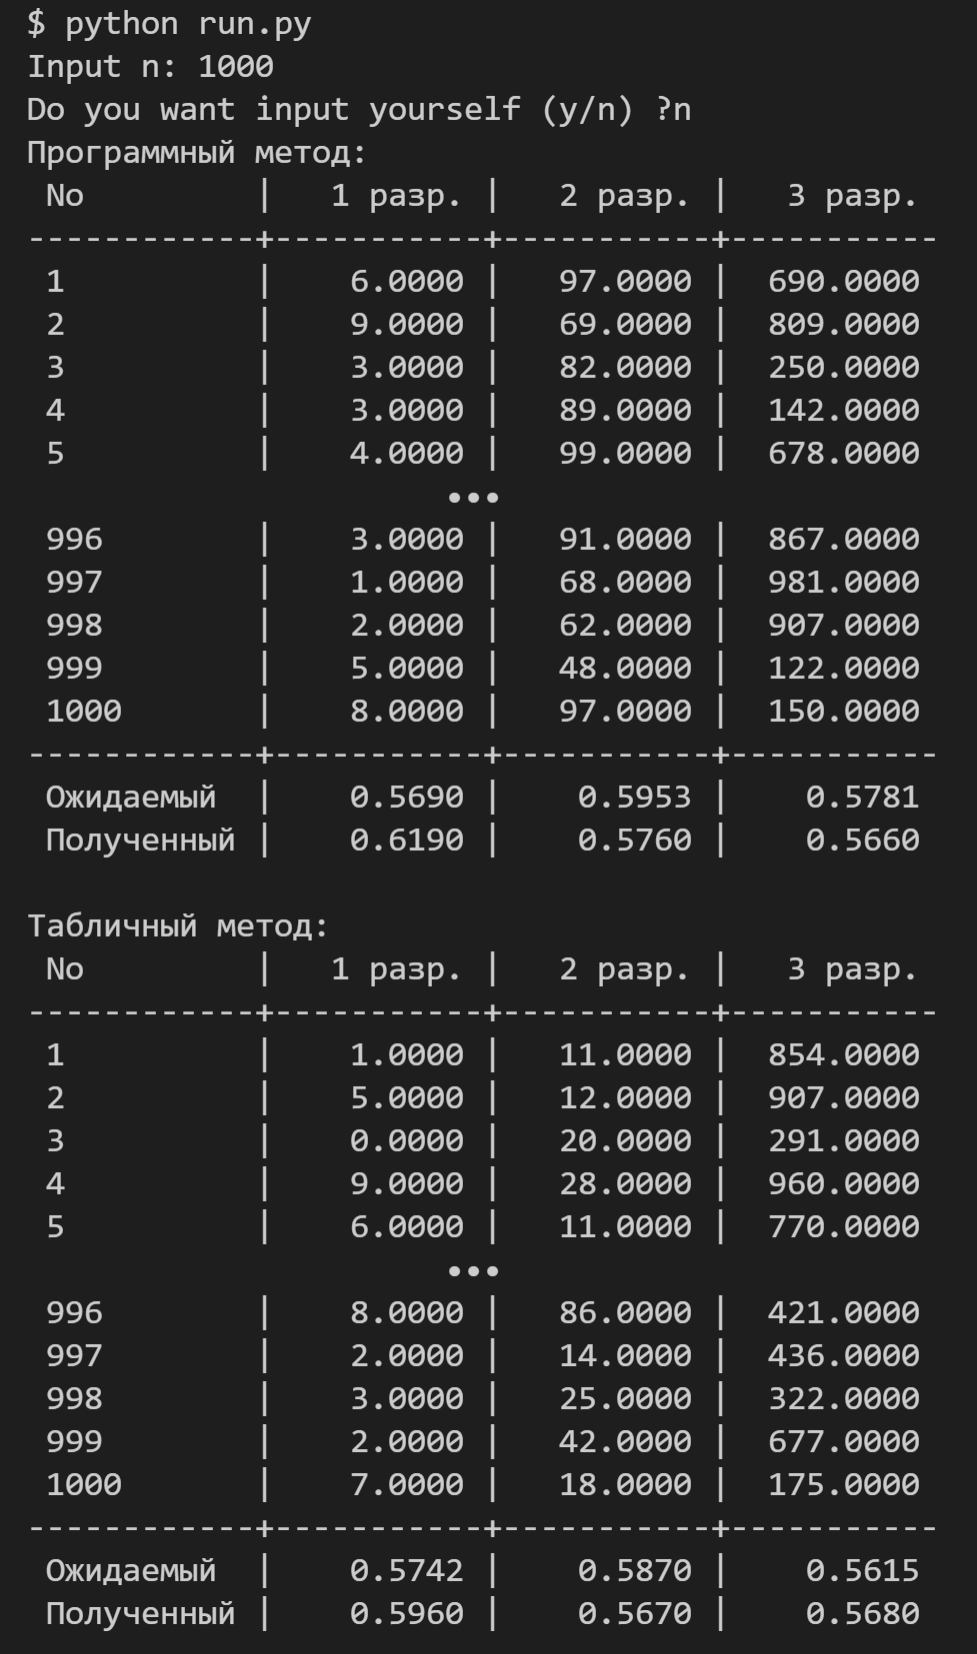
\includegraphics[scale=1]{1000}
	\centering\caption{Пример работы для 1000 чисел}
\end{figure}
\clearpage
\newpage
\section{Листинг кода}
\definecolor{codegreen}{rgb}{0,0.6,0}
\definecolor{codegray}{rgb}{0.5,0.5,0.5}
\definecolor{codepurple}{rgb}{0.58,0,0.82}
\definecolor{backcolour}{rgb}{0.95,0.95,0.92}

\lstdefinestyle{mystyle}{
	backgroundcolor=\color{backcolour},   
	commentstyle=\color{codegreen},
	keywordstyle=\color{magenta},
	numberstyle=\tiny\color{codegray},
	stringstyle=\color{codepurple},
	basicstyle=\ttfamily\footnotesize,
	breakatwhitespace=false,         
	breaklines=false,                 
	captionpos=b,                    
	keepspaces=true,                 
	numbers=left,                    
	numbersep=5pt,                  
	showspaces=false,                
	showstringspaces=false,
	showtabs=false,                  
	tabsize=4
}

\lstset{style=mystyle}

\begin{lstlisting}[language=Python, caption = Программная реализация генерации псевдослучайных чисел программным и табличным методом]
def frequency_criterion(sequence, num_len):
	mean = numpy.mean(sequence)
	stdd = numpy.sqrt(numpy.var(sequence))
	cnt = 0
	for item in sequence:
		if (mean - stdd) < item < (mean + stdd):
		cnt += 1
	
	sequence_max_delta = 10
	if num_len > 1:
		sequence_max_delta = 9 * 10**(num_len-1)
	
	return (2 * stdd / sequence_max_delta), (cnt /  len(sequence))


class StandardRandom():
	def get(self, num_len: int):
		return random.randint(10**(num_len - 1), 10**num_len)


class TableRandom():
	def __init__(self, path_to_table: str = "./table.txt"):
		self.digits = ""
		
		with open(path_to_table) as table_file:
			for line in table_file:
				self.digits += line[:-1]
		
		self.idx_init()
		
		def idx_step(self, step: int = 1):
			self.idx += step
		
		if self.idx + step >= len(self.digits):
			self.idx_init(step)
		
		def idx_init(self, offset: int = 0):
			now = datetime.datetime.now()
			self.idx = int((now.microsecond % 60)/60 * \\
						(len(self.digits) - offset))
		
		def get(self, num_len: int):
			self.idx_step(num_len)
			rnd_num = int(self.digits[self.idx:self.idx+num_len])
		
		while len(str(rnd_num)) < num_len:
			self.idx_step()
			rnd_num = rnd_num * 10 + int(self.digits[self.idx])

		return rnd_num
\end{lstlisting}
\section{Вывод}
\hspace*{5mm} Из результатов проведённой лабораторной работы справедливо сделать вывод, что, чем больше количество генерируемых случайных чисел, тем равномернее они распределены.
\end{document}